
\section{Numerical Methods for Fractional Differential Equations}

In this section we describe a numerical method which can be used to solve a fractional differential equation. We begin by looking at two ways for approximating a fractional derivative and then look at a specific scheme outlined by Diethelm \cite{Diethelm2011}.

\subsection{Approximations of Fractional Derivatives and Integrals}

\subsubsection{Gr\"{u}nwald-Letnikov Approximation}
In much the same was as we might use a finite difference method to approximate an integer order derivative we apply a similar approach here. By choosing some small, but non-zero value of $ h $ we can approximate the fractional derivative of a function by
\begin{align}
    \widehat{ \frac{d^\alpha f(t)}{dt^\alpha} } = \frac{1}{h^\alpha} \sum_{j=0}^n (-1)^j {\alpha \choose j} f(t - jh).
\end{align}

Also note that we have \emph{chopped} off the top of the series, taking on the first $ n $ terms in the sum. 
It can be shown \cite{Podlubny1999} that this yields a first order approximation of the Riemann-Liouville fractional derivative.
\subsubsection{Quadrature Approximation}
A completely different approach is to use a quadrature rule to evaluate the a fractional integral. This has particular utility when we wish to solve the equivelent integral equation.

There is no \emph{set way} to do the quadrature approximation and it will all depend on the scheme being used. 

In the following sections we will examine a general initial value problem and an Adams Moulton Bashforth scheme which is based off of a quadrature method. \cite{Diethelm2011}

\subsubsection{An Initial Value Problem}
Lets consider the initial value problem
\begin{align}
    \label{eq:num_ivp_1}
    \capder{0}{x}{\alpha}{y} &= f(x,y) \\
    \label{eq:num_ivp_2}
    y^{(k)}(0) &= y_{0}^{(k)} 
\end{align}
for $ 0 \leq k < \lfloor \alpha \rfloor $. Note that this initial value problem is stated in terms of Caputo derivatives. The motivation for such initial value problems was discussed in section \ref{subsec:caputo}.

One of the most important things to note about this equation is that for non-integer values of $ \alpha $ it is non-local, in the sense that the value of the solution at $ y(x_0+h) $ depends not only on $ y(x_0) $ but also on $ y(x), x \in [0, x_0] $ \cite{Diethelm2010}. This is in contrast to ordinary differential equations and this fact is what makes fractional differential equations considerably more complex to solve. Even multi-step methods which can be used to solve ordinary differential equations, only rely on some \emph{fixed} number previous time steps. As a solution to a fractional differential equation progresses it relies on more and more previous time steps. As one might suspect this fundamentally increases the computational complexity of the schemes used to solve fractional differential equations as compared with the schemes used to solve traditional ordinary differential equations. \footnote{It is possible to reduce these computations to look at some large but fixed number of previous grid-points 
but this results in a speed vs. accuracy tradeoff which will be discussed in section \ref{subsubsec:reduce_complexity}}

\subsubsection{The Adams Moulton Bashforth Scheme}
\label{sec:amb_desc}
We briefly outline a method explained and analysed in detail in \cite{Diethelm2004}. As shown in the proof of theorem \ref{thm:unique-tisdell} the initial value problem \eqref{eq:num_ivp_1}, \eqref{eq:num_ivp_2} is equivalent to the Volterra equation.

\begin{align}
    \label{eq:num_int_eq}
    y(x) = \sum_{k=0}^{\lceil \alpha \rceil - 1} y_{0}^{(k)} \frac{x^k}{k!} + \frac{1}{\Gamma(\alpha)} \int_0^x (x-t)^{\alpha - 1} f(t, y(t))dt
\end{align}
In order to approximate the solution to this integral equation over the interval $ [0, T] $, we select a number of grid points $ N $ so that $ h = T / N $ and $ x_k = hk $ where $ k \in \{0, 1, ..., N\} $.

We apply the approximation
\begin{align}
    \int_0^{x_{k+1}} (x_{k+1} - t)^{\alpha - 1} g(t)dt \approx \int_0^{x_{k+1}} (x_{k+1} - t)^{\alpha - 1} \tilde{g}_{k+1}(t)dt
\end{align}
where $ g(t) = f(t, y(t)) $ and $ \tilde{g}_{k+1}(t) $ is the piecewise linear approximation of $ g(t) $ with nodes at the grid-points $ x_k $. As outlined in \cite{Diethelm2004} we can approximate the integral in \eqref{eq:num_int_eq} as
\begin{align}
    \label{eq:amb_sum_1}
    \int_{0}^{x_{k+1}} (x_{k+1} - t)^{\alpha - 1} \tilde{g}_{k+1}(t) dt = \sum_{j=0}^{k+1} a_{j,k+1}g(x_j)
\end{align}
where 
\begin{align}
    a_{j,k+1} = \frac{h^\alpha}{\alpha(\alpha+1)} \times
    \begin{cases}
        (k^{\alpha+1}-(k-\alpha)(k+1)^\alpha) & \text{ if } j = 0 \\
        ((k-j+2)^{\alpha + 1} + (k-j)^{\alpha+1} - 2(k-j+1)^{\alpha+1}) & \text{ if } 1 \leq j \leq k \\
        1 & \text{ if } j = k + 1.
    \end{cases}
\end{align}

By separating the final term in the sum we can write
\begin{align}
\label{eq:amb_y_corr}
    y_{k+1} = \sum_{j=0}^{\lceil \alpha \rceil - 1} y_{0}^{(j)} \frac{x^j_{k+1}}{j!} + \frac{1}{\Gamma(\alpha)} \left( \sum_{j=0}^k a_{j,k+1} f(x_j,y_j) + a_{k+1,k+1}f(x_{k+1}, y_{k+1}^P )\right)
\end{align}
where $ y_{k+1}^P $ is a \emph{predicted} value for $ y_{k+1} $ which must be calculated due to the potential non-linearity of $ f $ \cite{Diethelm2004}.

This predicted value is calculated by taking a rectangle approximation to the integral in \eqref{eq:num_int_eq}, to get
\begin{align}
    \label{eq:amb_sum_2}
    \int_{0}^{x_{k+1}} (x_{k+1} - t)^{\alpha - 1} g(t) dt \approx \sum_{j=0}^k b_{j,k+1}g(x_j)
\end{align}
where
\begin{align}
    b_{j,k+1} = \frac{h^\alpha}{\alpha} \left( (k+1-j)^\alpha - (k-j)^\alpha \right).
\end{align}

and thus a predicted value of $ y_{k+1} $ can be calculated by
\begin{align}
    \label{eq:amb_y_pred}
    y_{k+1}^P = \sum_{j=0}^{\lceil \alpha \rceil - 1} \frac{x^{j}_{k+1}}{j!} y_{0}^{(j)} + \frac{1}{\Gamma(\alpha)} \sum_{j=0}^{k} b_{j,k+1} f(x_j, y_j).
\end{align}

This outlines a fractional Adams Moulton Bashforth scheme. Of particular note are the sums which arise in \eqref{eq:amb_sum_1} and \eqref{eq:amb_sum_2}. These sums do not arise in the integer order Adams Moulton Bashforth method. They arise as a result of the non-local nature of the fractional derivative \cite{Diethelm2004}. These sums represent a significant computational cost as the number of terms grow linearly as the solution progress. This means in the fractional case the Adams Moulton Bashforth method has computational complexity $ O(N^2) $ \cite{Diethelm2011}. Section \ref{sec:parallel_c} will outline a task based parallel approach and section \ref{sec:parallel_cuda} will outline a massively parallel approach to solving \eqref{eq:num_ivp_1}, \eqref{eq:num_ivp_2} with NVIDIA's CUDA.
\subsubsection{Parallelising: A Task Based Approach}
\label{sec:parallel_c}

Diethelm's paper \cite{Diethelm2011} outlines a parallel method of numerically approximating the solution to \eqref{eq:num_ivp_1}, \eqref{eq:num_ivp_2} by using a thread based parallel implementation of the Adams Moulton Bashforth method outlined in \ref{sec:amb_desc}. We base our approach in this section broadly on those of \cite{Diethelm2011} but reformulate the scheme in terms of tasks instead of threads. This has a number of distinct benefits including scalability, especially from an implementation standpoint and clarity.

After we have setup the grid-points $ x_0, \ldots, x_{N-1} $ we create an array of solution values $ y_0, \ldots, y_{N-1} $ which are to be populated with the calculated solution. From the initial conditions we can immediately calculate $ y_0 $. We then break up the vector (array) $ \mathbf{y} $ into blocks of size $ p $. Suppose that $ p = 2 $ for example. Then the first block would contain $ y_1 $ and $ y_2 $. Each of the $ p $ variables in each block can be calculated almost entirely in parallel. There is some dependency between values in each block (i.e. $ y_2 $ depends on $ y_1 $) but this can be done after the bulk of the parallel computations have been completed.

To illustrate this idea we consider figure \ref{fig:comp_diag}. We have broken the vector (array) $ \mathbf{y} $ up into $ K = \lceil \frac{N}{p} \rceil $ blocks of $ p $ variables.


\begin{figure}[h]
%AMB Y processing diagram

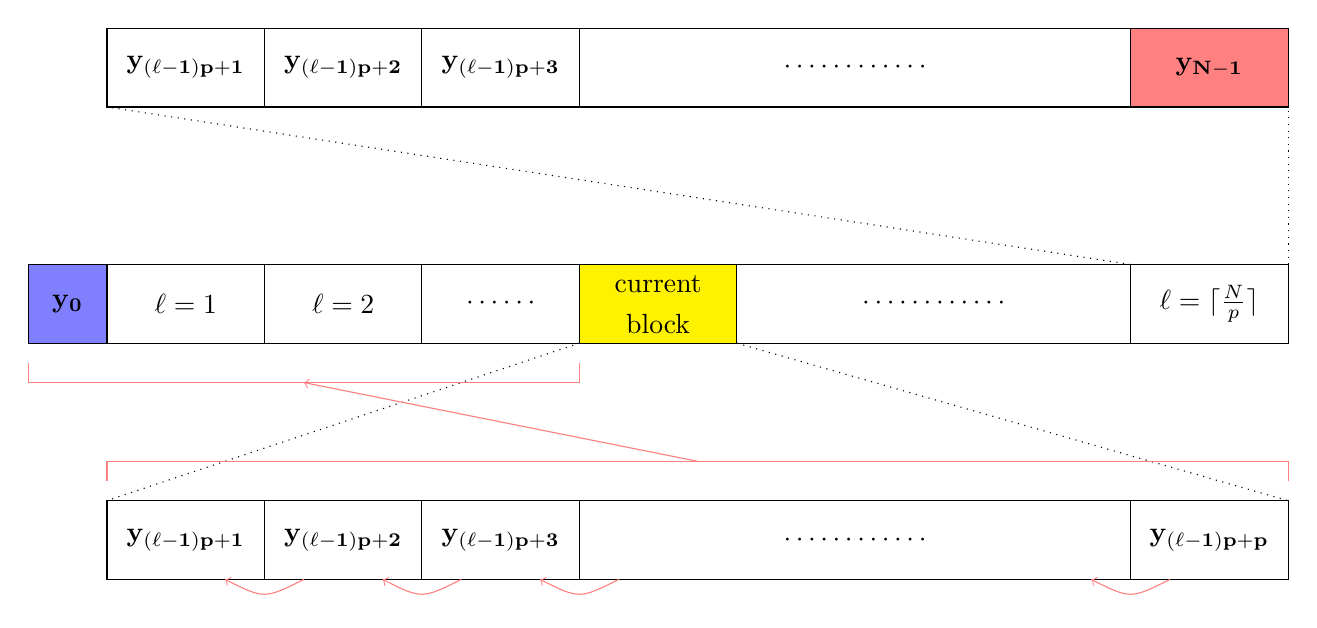
\begin{tikzpicture}
    \filldraw[fill=blue!50] (-1,0) rectangle (0,1);
    \draw (0,0) -- (0,1);
    \draw (-0.5,0.5) node { $ \mathbf{y_0} $ };
    \draw (-1,0) -- (15,0) -- (15, 1) -- (-1, 1) -- cycle;
    \draw (2,0) -- (2,1);
    \draw (4,0) -- (4,1);
    \draw (1,0.5) node { $ \ell = 1 $ };
    \draw (3,0.5) node { $ \ell = 2 $ };
    \draw (5,0.5) node { $ \cdots \cdots $ };
    \draw (6,0) -- (6,1);
    \draw (8,0) -- (8,1);
    \draw (10.5,0.5) node { $ \cdots \cdots \cdots \cdots  $ };
    \draw (13,0) -- (13,1);
    \draw (14,0.5) node { $ \ell = \lceil \frac{N}{p} \rceil $ };
    \filldraw[fill=yellow] (6,0) rectangle (8,1);
    \draw (7,0.75) node { current };
    \draw (7,0.25) node { block };
    \draw [dotted] (6,0) -- (0,-2);
    \draw [dotted] (8,0) -- (15,-2);
    \draw (0,-2) -- (15,-2) -- (15,-3) -- (0,-3) -- cycle;
    \draw (2,-3) -- (2,-2);
    \draw (4,-3) -- (4,-2);
    \draw (6,-3) -- (6,-2);
    \draw (13,-3) -- (13,-2);
    \draw (1,-2.5) node { $ \mathbf{ y_{(\ell - 1) p + 1} } $ };
    \draw (3,-2.5) node { $ \mathbf{ y_{(\ell - 1) p + 2} } $ };
    \draw (5,-2.5) node { $ \mathbf{ y_{(\ell - 1) p + 3} } $ };
    \draw (9.5, -2.5) node { $ \cdots \cdots \cdots \cdots $ };
    \draw (14,-2.5) node { $ \mathbf{ y_{(\ell - 1) p + p} } $ };
    \draw [dotted] (13,1) -- (0,3);
    \draw [dotted] (15,1) -- (15,3);
    \draw (0,3) -- (15,3) -- (15,4) -- (0,4) -- cycle;
    \draw (2,3) -- (2,4);
    \draw (4,3) -- (4,4);
    \draw (6,3) -- (6,4);
    \filldraw[fill=red!50] (13,3) rectangle (15,4);
    \draw (13,3) -- (13,4);
    \draw (1,3.5) node { $ \mathbf{ y_{(\ell-1)p + 1} } $ };
    \draw (3,3.5) node { $ \mathbf{ y_{(\ell-1)p + 2} } $ };
    \draw (5,3.5) node { $ \mathbf{ y_{(\ell-1)p + 3} } $ };
    \draw (9.5,3.5) node { $ \cdots \cdots \cdots \cdots $ };
    \draw (14,3.5) node { $ \mathbf{ y_{N-1} } $ };
    \draw [color=red!50, arrows={->}] (13.5,-3) .. controls (13,-3.25) .. (12.5,-3); 
    \draw [color=red!50, arrows={->}] (6.5,-3) .. controls (6,-3.25) .. (5.5,-3); 
    \draw [color=red!50, arrows={->}] (4.5,-3) .. controls (4,-3.25) .. (3.5,-3);    
    \draw [color=red!50, arrows={->}] (2.5,-3) .. controls (2,-3.25) .. (1.5,-3);
    \draw [color=red!50] (-1,-0.25) -- (-1,-0.5) -- (6,-0.5) -- (6,-0.25);
    \draw [color=red!50] (0,-1.75) -- (0,-1.5) -- (15,-1.5) -- (15,-1.75);
    \draw [color=red!50, arrows={->}] (7.5,-1.5) -- (2.5, -0.5);
\end{tikzpicture}

\caption{Computation diagram for the values in the vector (array) $ \mathbf{y} $.}
\label{fig:comp_diag}
\end{figure} 

The center row shows how $ \mathbf{y} $ is broken up into blocks, and the bottom row is a detailed view
of the contents of the \emph{current block} being computed.

The red lines indicate dependency, in that $ \mathbf{y}_{(\ell - 1)p + 1} $ depends on all the $ y_j $ values calculated in the previous blocks. $ \mathbf{y}_{(\ell - 1)p + 2} $ depends on all the $ y_j $ values calculated in previous blocks \emph{and} on $ \mathbf{y}_{(\ell - 1)p + 1 } $. 

The idea is that in each block we can do all of the computations which only depend on previous blocks in parallel and then perform the calculations which are dependent on other values within the same block in sequence. After all the values in a particular block are calculated we move on to the next block and repeat the process.

An exploded view of the last block is also provided to emphasize the fact that this block might not contain $ p $ variables if $ p $ does not divide $ N - 1 $. This fact causes us no bother as it is easy to handle in code.

As in \cite{Diethelm2011} we rewrite the equations \eqref{eq:amb_y_corr} and $ \eqref{eq:amb_y_pred} $ as
\begin{align}
y_{j+1}^P = I_{j+1} + h^\alpha H_{j,\ell}^P + h^\alpha L_{j,\ell}^P
\end{align}
and
\begin{align}
y_{j+1} = I_{j+1} + h^{\alpha} H_{j,\ell} + h^\alpha L_{j,\ell}
\end{align}

where
\begin{align}
I_{j+1} & := \sum_{k=0}^{\lceil \alpha \rceil -1} \frac{x_{j+1}^k}{k!} y_0^{(k)} \\
H^P_{j,\ell} & := \sum_{k=0}^{(\ell-1)p} b_{j-k} f(x_k, y_k) \\
L_{j,\ell}^P & := \sum_{k=(\ell-1)p+1}^{j} b_{j-k} f(x_k,y_k) \\
H_{j,\ell} & := c_j f(x_0, y_0) + \sum_{k=1}^{(\ell - 1)p} a_{j-k}f(x_k, y_k) \\
L_{j,\ell} & := \sum_{k=(\ell-1)p + 1}^j a{j-k} f(x_k, y_k) + \frac{f(x_{j+1}, y^P_{j+1})}{\Gamma(\alpha + 2.)}
\end{align}

In each block the values of $ H, I $ and $ H^P $ can be calculated in parallel for each $ y_j $ in the block.Then there is a somewhat more complex dependency between these sums. 

To best explain how the processes proceeds in each block and what dependencies there are we will consider a specific example where there are two values to be calculated per block (i.e. $ p = 2 $). Consider figure \ref{fig:AMB_Task_Flow}. 

Each box in the figure represents a task. A task can execute when all the tasks with arrows pointing to it have completed. The little red number represents the index of the variable \emph{within} the block which is being calculated. All the task names are reasonably self explanatory except for perhaps $ S^P $ and $ S $. These take the values calculated in the other sums and add them together to get $ y^P $ and $ y $ respectively. These are very small tasks which take very little time to execute.

The red arrow illustrate the interdependency of variables within a block. The second variable cannot have the sum $ L^P $ calculate until the first variable is calculated. This means that in effect each of the $ L $ tasks have to execute in series but these sums are relatively small so the time taken is quite short. Each block is then executed in sequence as each block depends on the blocks before it. See Appendix A for a C\# implementation of this. 

\begin{figure}[H]
%PID Controller Closed Loop Diagram.
\begin{tikzpicture} 
    \draw (10,20) -- (13,20) -- (13, 19) -- (10, 19) -- cycle;
    \draw (11.5,19.5) node { Block Start };
    \draw (11.5, 19) -- (11.5, 18);
    \draw (4.5, 18) -- (19.5, 18);
    \draw [->] (4.5, 18) -- (4.5, 17);
    \draw [->] (7.5, 18) -- (7.5, 17);
    \draw [->] (10.5, 18) -- (10.5, 17);
    \draw [->] (11.5, 18) -- (11.5, 13) -- (10, 13);
    \draw (3.75, 17) -- (5.25, 17) -- (5.25, 15.5) -- (3.75, 15.5) -- cycle;
    \draw (6.75, 17) -- (8.25, 17) -- (8.25, 15.5) -- (6.75, 15.5) -- cycle;
    \draw (9.75, 17) -- (11.25, 17) -- (11.25, 15.5) -- (9.75, 15.5) -- cycle;
    \draw (8.5, 12.25) -- (10, 12.25) -- (10,13.75) -- (8.5, 13.75) -- cycle;
    \draw (7.5, 14.5) -- (10.5, 14.5);
    \draw [->] (4.5, 15.5) -- (4.5, 4.25) -- (8.5, 4.25);
    \draw (7.5, 14.5) -- (7.5, 15.5);
    \draw (10.5, 14.5) -- (10.5, 15.5);
    \draw (7.5, 15.5) -- (7.5, 10);
    \draw [->] (7.5, 10) -- (8.5, 10);
    \draw (8.5, 9.25) -- (8.5, 10.75) -- (10, 10.75) -- (10, 9.25) -- cycle;
    \draw [->] (9.25, 12.25) -- (9.25, 10.75);
    \draw [->] (9.25, 9.25) -- (9.25, 8);
    \draw (8.5, 8) -- (10, 8) -- (10, 6.5) -- (8.5, 6.5) -- cycle ;
    \draw [->] (9.25, 6.5) -- (9.25, 5);
    \draw (8.5, 5) -- (8.5, 3.5) -- (10, 3.5) -- (10, 5) -- cycle;
    \draw [->] (18.5, 18) -- (18.5, 17);
    \draw [->] (15.5, 18) -- (15.5, 17);
    \draw [->] (12.5, 18) -- (12.5, 17);
    \draw (11.75, 17) -- (13.25, 17) -- (13.25, 15.5) -- (11.75, 15.5) -- cycle;
    \draw (14.75, 17) -- (16.25, 17) -- (16.25, 15.5) -- (14.75, 15.5) -- cycle;
    \draw (17.75, 17) -- (19.25, 17) -- (19.25, 15.5) -- (17.75, 15.5) -- cycle;
    \draw [->] (12.5, 15.5) -- (12.5, 4.25) -- (16.5, 4.25);
    \draw [->] (19.5, 18) -- (19.5, 13) -- (18, 13);
    
    
    \draw (15.5, 14.5) -- (18.5, 14.5);
    \draw [->] (12.5, 15.5) -- (12.5, 4.25) -- (16.5, 4.25);
    \draw (15.5, 14.5) -- (15.5, 15.5);
    \draw (18.5, 14.5) -- (18.5, 15.5);
    \draw (15.5, 15.5) -- (15.5, 10);
    \draw [->] (15.5, 10) -- (16.5, 10);
    \draw (16.5, 9.25) -- (16.5, 10.75) -- (18, 10.75) -- (18, 9.25) -- cycle;
    \draw [->] (17.25, 12.25) -- (17.25, 10.75);
    \draw [->] (17.25, 9.25) -- (17.25, 8);
    \draw (16.5, 8) -- (18, 8) -- (18, 6.5) -- (16.5, 6.5) -- cycle ;
    \draw [->] (17.25, 6.5) -- (17.25, 5);
    \draw (16.5, 5) -- (16.5, 3.5) -- (18, 3.5) -- (18, 5) -- cycle;
    \draw (16.5, 12.25) -- (18, 12.25) -- (18,13.75) -- (16.5, 13.75) -- cycle;
    \draw [color=red, arrows={->}] (10, 4.25) -- (12,4.25) -- (12, 13) -- (16.5, 13);
    \draw (4.5, 16.25) node { $ H $ };
    \draw (5, 15.75) node[color=red]  { $ 1 $ };
    
    \draw (7.5, 16.25) node { $ I $ };
    \draw (8, 15.75) node[color=red]  { $ 1 $ };
    
    \draw (10.5, 16.25) node { $ H_p $ };
    \draw (11, 15.75) node[color=red]  { $ 1 $ };
    
    \draw (9.25, 13) node { $ L_p $ };
    \draw (9.75, 12.5) node[color=red] { $ 1 $ };
    
    \draw (9.25, 10) node { $ S_p $ };
    \draw (9.75, 9.5) node[color=red] { $ 1 $ };
    
    \draw (9.25, 7.25) node { $ L $ };
    \draw (9.75, 6.75) node[color=red] { $ 1 $ };
    
    \draw (9.25, 4.25) node { $ L $ };
    \draw (9.75, 3.75) node[color=red] { $ 1 $ };
    
    
    
    \draw (12.5, 16.25) node { $ H $ };
    \draw (13, 15.75) node[color=red]  { $ 2 $ };
    
    \draw (15.5, 16.25) node { $ I $ };
    \draw (16, 15.75) node[color=red]  { $ 2 $ };
    
    \draw (18.5, 16.25) node { $ H_p $ };
    \draw (19, 15.75) node[color=red]  { $ 2 $ };
    
    \draw (17.25, 13) node { $ L_p $ };
    \draw (17.75, 12.5) node[color=red] { $ 2 $ };
    
    \draw (17.25, 10) node { $ S_p $ };
    \draw (17.75, 9.5) node[color=red] { $ 2 $ };
    
    \draw (17.25, 7.25) node { $ L $ };
    \draw (17.75, 6.75) node[color=red] { $ 2 $ };
    
    \draw (17.25, 4.25) node { $ L $ };
    \draw (17.75, 3.75) node[color=red] { $ 2 $ };
    
    \draw [->] (17.25, 3.5) -- (17.25, 2) -- (11.5, 2) -- (11.5, 1);
    
    \draw (10,1) -- (13,1) -- (13, 0) -- (10, 0) -- cycle;
    \draw (11.5,0.5) node { Block End };
\end{tikzpicture}

\caption{Task flow diagram for each block in the case when $ p = 2 $}
\label{fig:AMB_Task_Flow}
\end{figure}

\subsubsection{Analysis of the Performance of the Scheme in C\# and MONO}

We wish to analyze the performance of this scheme both from a theoretical standpoint and from at practical standpoint. 

For the theoretical analysis of the scheme we introduce Amdahl's Law or Amdahl's principle.
\begin{mdframed}[innertopmargin=10pt]
\begin{principle}[Amdahl]
Let $ P $ be the proportion of a computation which can be parallelised in a given progress. Then the speedup given by
$ Q $ cores is
\begin{align}
	S(Q) = \frac{1}{(1-P)+\frac{P}{Q}}
\end{align}

\end{principle}
\end{mdframed}

This law was first introduced in a 1967 paper by computer architect Amdahl. We introduce a new notion of Amdahl efficiency to characterize the how \emph{good} a parallel algorithm is in comparison with it serial counterpart in the limit of large input. 

To formalize this notion we introduce the following definition.
\begin{mdframed}[innertopmargin=10pt]
\begin{definition}[Amdahl Efficiency]
\label{def:amdahl_efficient}
    Let $ S(N,Q) $ represent the parallel speedup for a problem with input size $ N $ and executed with $ Q $ cores.
    Then we define the Amdahl efficiency of parallel scheme as 
    \begin{align}
        E(Q) = \lim_{N \lra \infty} \frac{S(N, Q)}{Q}.
    \end{align}
    Further we say that a parallel scheme is Amdahl efficient with respect to its serial counterpart if $ E(p) = 1 $.
\end{definition}
\end{mdframed}

\begin{mdframed}[innertopmargin=10pt]
\begin{proposition}
The parallel Adams Moulton Bashforth scheme is Amdahl efficient with respect to its serial counterpart.
\end{proposition}
\end{mdframed}
\begin{proof}
We present the paralellizable fraction of computation in each block of variables in the following table. The order column represents the number of \emph{multiply-add} operations per task.

\begin{tabular}[ht]{|c|c|c|c|}
\hline
Task        & Computational Complexity  & Number of Variables per Block     & Total Complexity \\ \hline
$ H $       & $ O(\ell p ) $            & $ p $                             & $ O(\ell p^2) $ \\ \hline
$ H_p $     & $ O(\ell p ) $            & $ p $                             & $ O(\ell p^2) $ \\ \hline
$ I $       & $ O( \alpha ) $           & $ p $                             & $ O(p) $ \\ \hline \hline          
$ L $       & $ O( p ) $                & $ p $                             & $ O(p^2) $ \\ \hline
$ L_p $     & $ O( p ) $                & $ p $                             & $ O(p^2) $ \\ \hline
\end{tabular}

In each block $ H $, $ H_p $ and $ I $ can be computed in parallel across all variables in the block. For the purposes of simplicity we assume that the tasks $ L $ and $ L_p $ must all be computed in serial across all variables in a block. This means that in the $ \ell$-th block the non-paralellizable fraction of computation is
\begin{align}
    \overline{P}_{block}(\ell) \sim \frac{2p^2}{2p^2(\ell + 1) } \sim \frac{1}{\ell}
\end{align}

The amount of computation in the $ \ell$-th block is $ O(\ell p^2) $ and there are $ K \approx \frac{N}{p} $ blocks in the total computation. This means that the total amount of computation is
\begin{align}
    \sum_{\ell=1}^{K} \ell p^2 \sim \frac{K^2p^2}{2}
\end{align}
and by taking a weighted average sum, the total fraction of non-paralellizable computation is
\begin{align}
    \label{eq:tot_par_c}
    \overline{P}_{total} \sim \sum_{\ell = 1}^{K} \frac{2\ell p^2}{K^2 \ell p^2} = \frac{2}{K} = \frac{2p}{N}.
\end{align}

Noticing the fact that the computation in the task $ I $ is insignificant compared to $ H $ and $ H_p $ we would suppose using $ Q = 2p $ cores would be in some sense optimal. Applying Amdahl's principle with the result in \ref{eq:tot_par_c} and with $ Q = 2p $ we get 
\begin{align}
    S(N, Q) &= S(N, 2p) \\
    &\sim \frac{1}{(\frac{2p}{N}) + \frac{1-\frac{2p}{N}}{2p} } \\
\end{align}
then letting $ N \lra \infty $ we get
\begin{align}
    E(p) = \lim_{N \lra \infty} \left(\frac{1}{(\frac{2p}{N}) + \frac{1-\frac{2p}{N}}{2p} } \right) \slash p = 1.
\end{align}

\end{proof}

What this result means is that if we have $ 2p $ free cores this parallel method should take $ \frac{1}{2p} $ the amount of time to run compared to its serial counterpart given a sufficiently large number of grid points, $N$. Due to the fact that this a task based scheme this is also dependent on an efficient scheduler.

We now compare this with practical experimentation. This method was developed in C\# with MONO (see Appendix A for C\# code) and run on a machine with an Intel \textregistered Core \texttrademark{} i7-4930K CPU @ 3.40GHz. This particular CPU has 6 physical cores with 12 logical cores provided by hyper-threading. 

We solved the following initial value problem

\begin{align}
    \capder{0}{x}{\frac{1}{2}}{y}(x) = -y(x) & & y(0) = 1
\end{align}

with $ N = 2000 $ through to $ N = 10000 $ time steps over the interval $ [0,10] $ with $ p $ ranging from $ 1 $ though to $ 12 $. Each solution was computed 5 times and the average runtime  was computed, yielding the \emph{performance surface} shown in figure \ref{fig:mono_performance_surface}. \footnote{See Appendix B for a full table of runtimes.}

\begin{figure}[H]
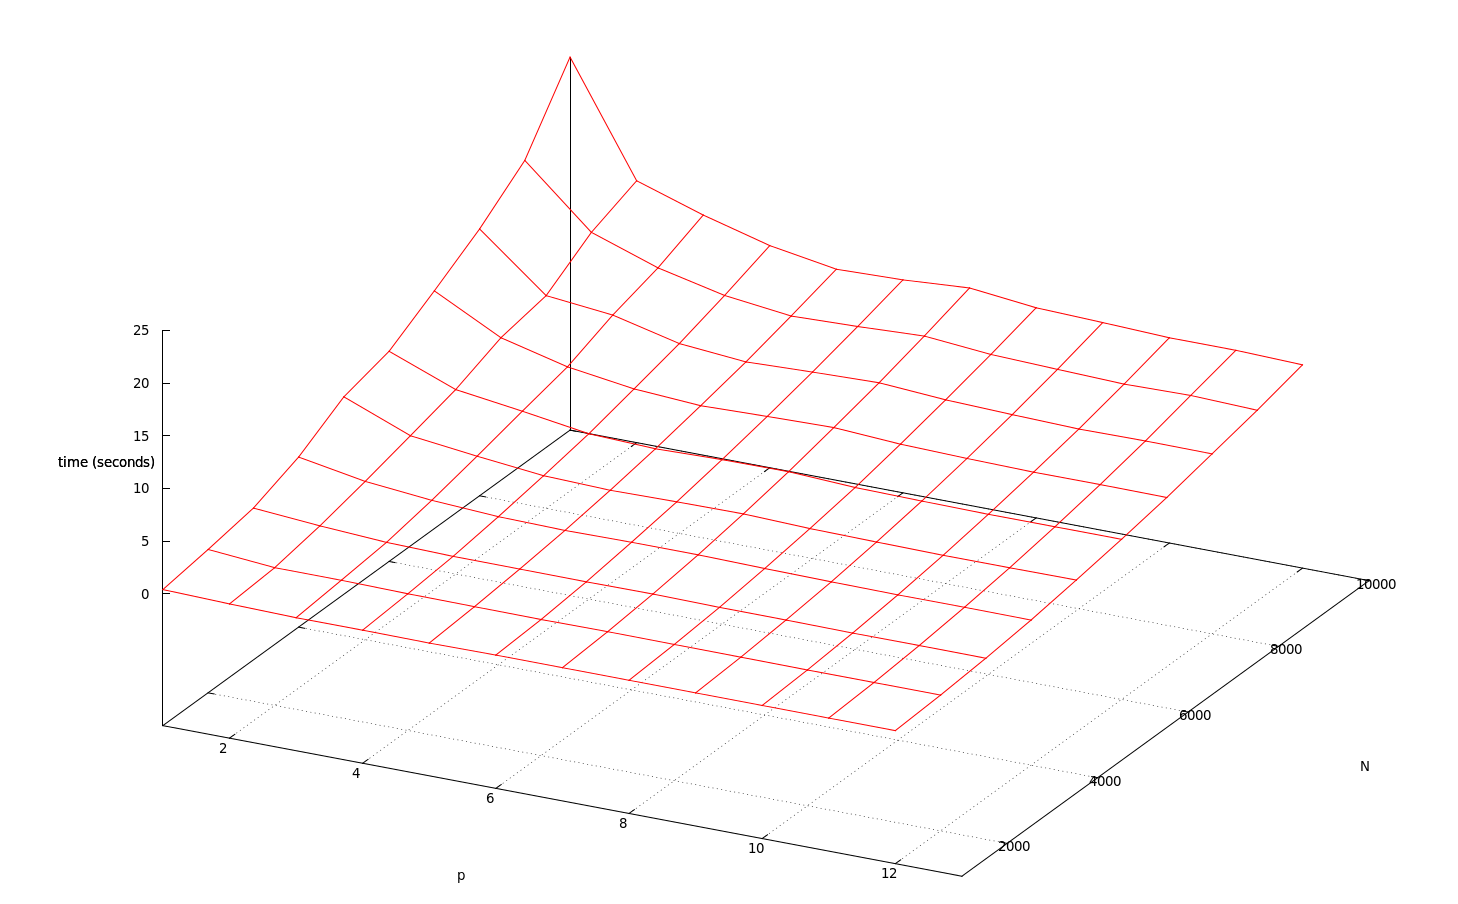
\includegraphics[scale = 0.3]{images/Dot_Net_Performance_No_Label}
\caption{Average runtime of the scheme for different values of $ p $ and $ N $. }
\label{fig:mono_performance_surface}
\end{figure}

Figure \ref{fig:mono_performance_surface} clearly shows the $ O(N^2) $ complexity of the algorithm, especially in the case where $ p = 1 $. 
We present some of the results from the $ N = 10000 $ computations in a figure \ref{tab:mono_speedup} to illustrate the speedup. 
\begin{figure}[h]
\label{tab:mono_speedup}
\begin{tabular}[ht]{|c|c|c|}
\hline
p       & Runtime (s)   & Speedup (wrt p = 1)\\ \hline
1       & 22.89         & 1  \\ \hline
2       & 12.35         & 1.85 \\ \hline
3       & 10.28         & 2.22 \\ \hline
4       & 8.58          & 2.66 \\ \hline
5       & 7.53          & 3.04 \\ \hline
6       & 7.70          & 2.97 \\ \hline
\end{tabular}
\end{figure}

From a theoretical perspective we would expect speedups of 2, 3 and 4 for the cases $ p =2,3, 4 $ respectively, however, this is not achieved. There are a number of possible reasons for this. Firstly the MONO task scheduler (based of the .Net scheduler) is not performance optimized \cite{MicrosoftTaskSchedular}.

There is the possibility that we haven't chosen a large enough value of $ N $ to get the full relative speedup. This is supported by the fact that for the $ N = 8000 $ case the speedup from $ p = 1 $ to $ p = 2 $ was $ 1.53 $ (less than that in the $ N = 10000 $ case). 

Also for cases where $ p > 3 $ we have 6 computationally heavy tasks ( $ H $ and $ H_p $ ) being completed per block and are therefore reaching the limit of the number of physical cores on the system. Obviously we cannot expect an improvement once $ p $ gets too large as the number of tasks to be executed in parallel exceeds the number of available cores. We see the full effect of this in the $ p = 6 $ case where the runtime was actually longer than that for $ p = 5 $.

\subsubsection{Parallelising: A CUDA Approach}

\label{sec:parallel_cuda}

One of the main benefits of the scheme outlined in section \ref{sec:parallel_c}, especially noted in it's form presented by Diethelm in \cite{Diethelm2011} is the ability for this scheme to be implemented across multiple machines with a small amount of message passing between executing threads (or in this case tasks). The main reason for wanting to minimize message passing is that it can significantly impact performance to the point where most of the time is actually spent communicating updates between execution nodes. This is given significant consideration in \cite{Diethelm2011}. In this section we abandon these measures in favour of massive performance gains when executing in a massively parallel manner on a GPU.

Modern graphics cards have the advantage of being able to efficiently perform massively parallel computations, especially calculations involving floating point arithmetic \cite{Fernando2005}. For example the NVIDIA GeForce GTX 780 has 2304 cores clocked at 863MHz. We use one of these graphics cards in an effort to dramatically speed up the fractional Adams Moulton Bashforth Method using NVIDIA's CUDA tool-chain.

Instead of using blocks of variables as was done in \cite{Diethelm2011} and reimplemented by us in section \ref{sec:parallel_c} we return to the original specification of the scheme in section \ref{sec:amb_desc} and seek out other opportunities of parallelism.

The essential problem with the scheme is that the number of terms in the sums defined in \eqref{eq:amb_y_pred} and \eqref{eq:amb_y_corr} grows linearly with each time step taken. It is clear that the actual terms in each sum are independent and so breaking the sum up into smaller parts to be calculated and then summed together is a reasonable approach. This is so long as communication between cores doing different parts of the sum is sufficiently fast and global memory access is sufficiently fast. In the case of a GPU both of these criteria are satisfied and so this approach is reasonable.\footnote{It is easy to see that this scheme would be Amdahl efficient in the sense of definition \ref{def:amdahl_efficient}.}

We aim to use as much of the GPU as possible to perform the calculations and so unlike the scheme outlined in section \ref{sec:parallel_c} we will automatically scale the number of threads to use as many cores as possible. We define one \emph{performance tuning} parameter $ opsPerThread $ which define the number of \emph{multiply-add} operations per thread. 
Figure \ref{fig:cuda_performance_surface} shows a \emph{performance surface} showing runtime against number of time steps $ N $ and $ opsPerThread $ \footnote{See appendix B for a full table of runtimes}. The actual initial value problem being solved is exactly the same as in section \ref{sec:parallel_c}.

\begin{figure}[H]
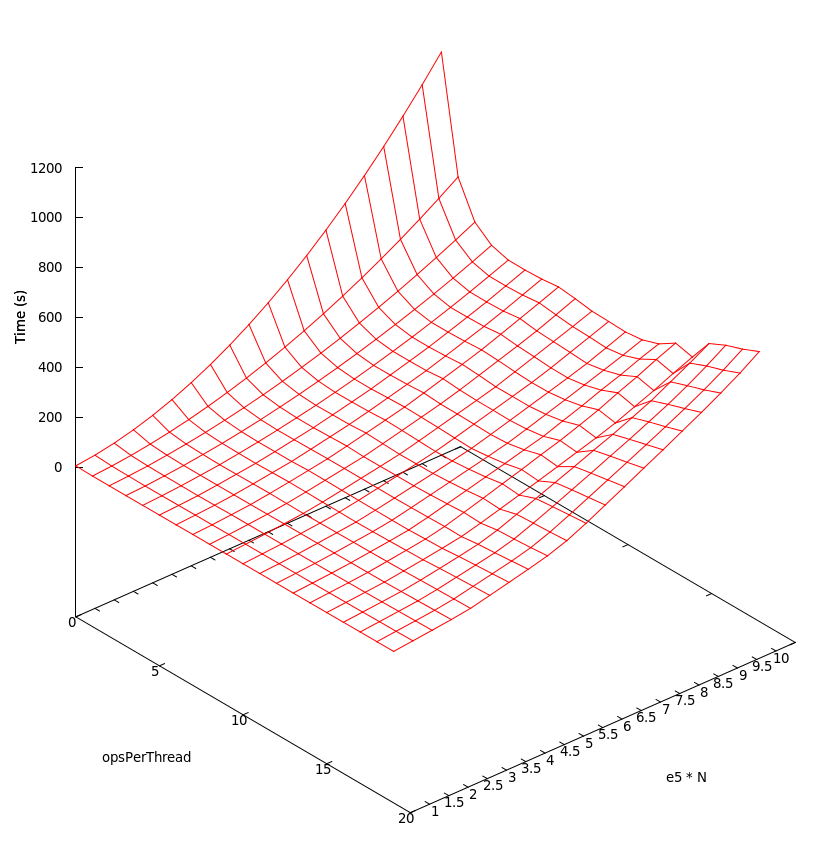
\includegraphics[scale = 0.4]{images/CUDA_Performance_No_Label}
\caption{Runtime for the scheme for various values of opsPerThread and N.}
\label{fig:cuda_performance_surface}
\end{figure}

Firstly we note the size of the problems being solved here. The last point on the $ N $ axis is $10^6$ time-steps, 100 times larger than was computed in the CPU based C\# approach. Given the quadratic computational complexity of this algorithm that means this CUDA implementation is solving problems which would take roughly $ 2.5 $ days to compute using the previous parallel scheme, in less than 6 minutes.

As can be seen from this chart, as $ N $ increases it makes sense to perform more operations per thread. This arises from the fact that there is an overhead in dealing with each thread and this overhead becomes significant as $ N $ gets large. This effect is also exacerbated by the fact that for small values of $ N $ the overhead of managing more threads on the GPU is offset by the increased parallelism that a smaller number of operations per thread affords. Once, however, every core is being utilized it makes sense to start to increase the number of operations per thread as $ N $ is increased.

The speedup from running these computation on CUDA is enormous. It is arguable that any advantage achieved through reducing the number of messages passed between multiple threads and nodes by using the scheme outlined in \cite{Diethelm2011} and in section \ref{sec:parallel_c}, is completely outweighed by the sheer speed of computation on a GPU. 

\subsubsection{Short Memory Principle}
\label{subsubsec:reduce_complexity}

We can actually completely change the complexity class of the problem by improving our solution so as to take advantage of the so-called \emph{short memory principle}.  \cite{Podlubny1999, Ford2001}.

The most basic approach is the fixed memory principle as outlined in \cite{Podlubny1999} and again in \cite{Ford2001}. The idea is to truncate the integral in the equivalent integral equation, such as in \label{eq:num_int_eq}. We would like to characterise the trade off in terms of accuracy that occurs when one takes this approach. That is, how much accuracy is sacrificed for different \emph{look back} lengths.

For simplicity let's consider $ \alpha \in (0, 1) $ and let's consider the Caputo fractional derivative of some admissible function $ f $.
We wish to approximate
\begin{align}
	\frac{1}{\Gamma(1-\alpha)} \int_0^t \frac{f'(t)}{(t-s)^\alpha} ds
\end{align}
by
\begin{align}
	\frac{1}{\Gamma(1-\alpha)} \int_{({t-T})\vee 0}^t \frac{f'(t)}{(t-s)^\alpha} ds
\end{align}
where $ T $ is essentially some \emph{lookback length}.
The difference between these two integrals is 
\begin{align}
	\left| \frac{1}{\Gamma(1-\alpha)} \int_0^t \frac{f'(t)}{t-s)^\alpha} ds - \frac{1}{\Gamma(1-\alpha)} \int_{t-T}^t \frac{f'(t)}{t-s)^\alpha} ds \right| =  \left| \frac{1}{\Gamma(1-\alpha)} \int_{0}^{({t-T})\vee 0} \frac{f'(t)}{(t-s)^\alpha} ds \right|
\end{align}
which we refer to as the truncation error, $E$. So long as $ f' $ is bonded (by say $ M $) on some interval $ [0,a] $ then we can say that 
\begin{align}
	E &\leq \frac{M}{\Gamma(1-\alpha)} \int_0^{({t-T})\vee 0} \frac{1}{(t-s)^\alpha} ds| \\
		&= \left(\frac{M}{\Gamma(2 - \alpha)} (t^{1-\alpha} - T^{1-\alpha})\right)\vee 0
\end{align}
on $ [0,a] $.
As noted in \cite{Ford2001} such an approach would result in a loss of order. If we insist that $ E \leq \varepsilon $ then we would have to choose T such that
\begin{align}
	T^{1-\alpha} \geq t^{1-\alpha} - \left( \frac{\varepsilon \Gamma(2 - \alpha)}{M}\right).
\end{align}
As noted in \cite{Ford2001} it turns out that such a requirement essentially removes any computational benefit from truncating the integral so although such a technique would reduce the complexity of each step to $ \mathcal{O}(1) $ and hence the overall complexity to $ \mathcal{O}(n) $ we would be making significant accuracy trade-offs.

\subsubsection{Nested Mesh Technique}

Another technique which could reduce the computational complexity of the problem is the so called \emph{nested mesh technique}. This technique is also well known and a good explanation of it is given by Ford \cite{Ford2001}. The basic idea is to change the step-size for the approximation of the integral across different parts of the integral. Specifically it would mean logarithmically increasing the step size for the quadrature approximation of the integral for points further back in time. 


\clearpage 
